\section{Preparing the ground for another camp}
\margininbox{Republika}{
     \begin{citemize}
     \item Jarvist Frost
    \item Rhys Tyers
    \end{citemize}
}{\explo}

\paragraph{Prelude}
With a new job in Bath, yet still one half of my life in London, I hurtled towards the summer with some severe time restrictions and I feared that I would not be able to make it to the expedition. \bignote{After some time staring into my soul, I withdrew an abstract from a conference and booked some cheap flights Bristol to Treviso}. All I could line up was ten days, 25th July to the 4th August.

I made it to London the weekend before the van left, and joined in with the last minute preparations -- pushing trolleys around Clapham Lidl and ASDA, filling our boots with cut price carbohydrates and ready munch. We then had a full day in stores, helping deal with the too-long and yet ill-defined and nebulous to-do list. A big oversight was that the underground camp gear had remained unwashed since the previous summer, and so required many hours of laundry room attendance as the sleeping bags and comf were washed and then extensively tumble dried before being packed for -550 m.

My drone (a Husban H107C HD Camera quadcopter) arrived in time to be sealed in a mini Daren drum with my XML bike light, but not much tested. It fits wonderfully in a small Daren drum with a few roll-mat circles of padding. The controller actually clips within the bottom ring, and the rotor cage of the quadcopter similar sits gently against the narrowing for the neck.


\begin{marginfigure}
\checkoddpage \ifoddpage \forcerectofloat \else \forceversofloat \fi
\centering
 \frame{\includegraphics[width=\linewidth]{"images/2014/jarv-2014/jan_ravne".jpg}} 
 \caption{The hiking trail leading to \protect\passage{Tolminski Migovec} starts a \protect\passage[hamlet]{Ravne} \pic{Jan Evetts}}
 \label{quadcopter}
\end{marginfigure}


\paragraph{Arrival}

The flight out was pleasant, but I had a lot of travelling to do in Europe. From Treviso I walked to the train station to catch one of the every two-hour trains towards Gorizia. Jackie's pub, just near the airport, served good pizza on the way back. From Treviso I trained to Gorizia, caught the 1-Euro international bus across the border to Nova Gorica (bus station), and then caught the evening bus to Tolmin. I arrived in time to meet Tetley, Martin, Janet and friend, and go out for Pizza.

The next morning, Janet had very kindly offered to get up early (6:30!) and drive us to \passage{Ravne} in her hire car. This was a great boon, and two carries later I was firmly ensconced upon the mountaintop. Unfortunately, my timings did not mesh with the expedition. Many people were leaving that weekend, and so most cavers headed down to Tolmin. I spent my time on Sunday doing a food carry, and generally fettling. The weather during my time there was appalling -- almost no sun, clag or heavy rain the rest of the time. At least it was fairly warm!

Rhys had returned, and we had a plan to go caving (a 3 day camp) on Tuesday, which would form the totality of my expedition. The weather was horrific, rain and clag which made it difficult to muster the enthusiasm to go caving, or to prepare gear and pack Daren drums. We decided to rotate onto the Night Train (i.e. sleep during the day) due to our slipping timings, and to make more considerate use of the 4-bed camp at \passage{X-Ray}. We had a hare-brained plan to setup a full blown mini camp at \passage{Red Cow}, but the amount we would have to take down (and take out) was prohibitive; and there were no more club 4-season sleeping bags so would be very cold. There was also the obvious safety implications of camping away from the others, with potentially no contact for days (i.e. no daily callout). Dan Greenwald had done a bounce trip to \passage{X-Ray} on Monday, replenishing the camp with supplies and removing rubbish.

\begin{marginsurvey}
\checkoddpage \ifoddpage \forcerectofloat \else \forceversofloat \fi
\centering
 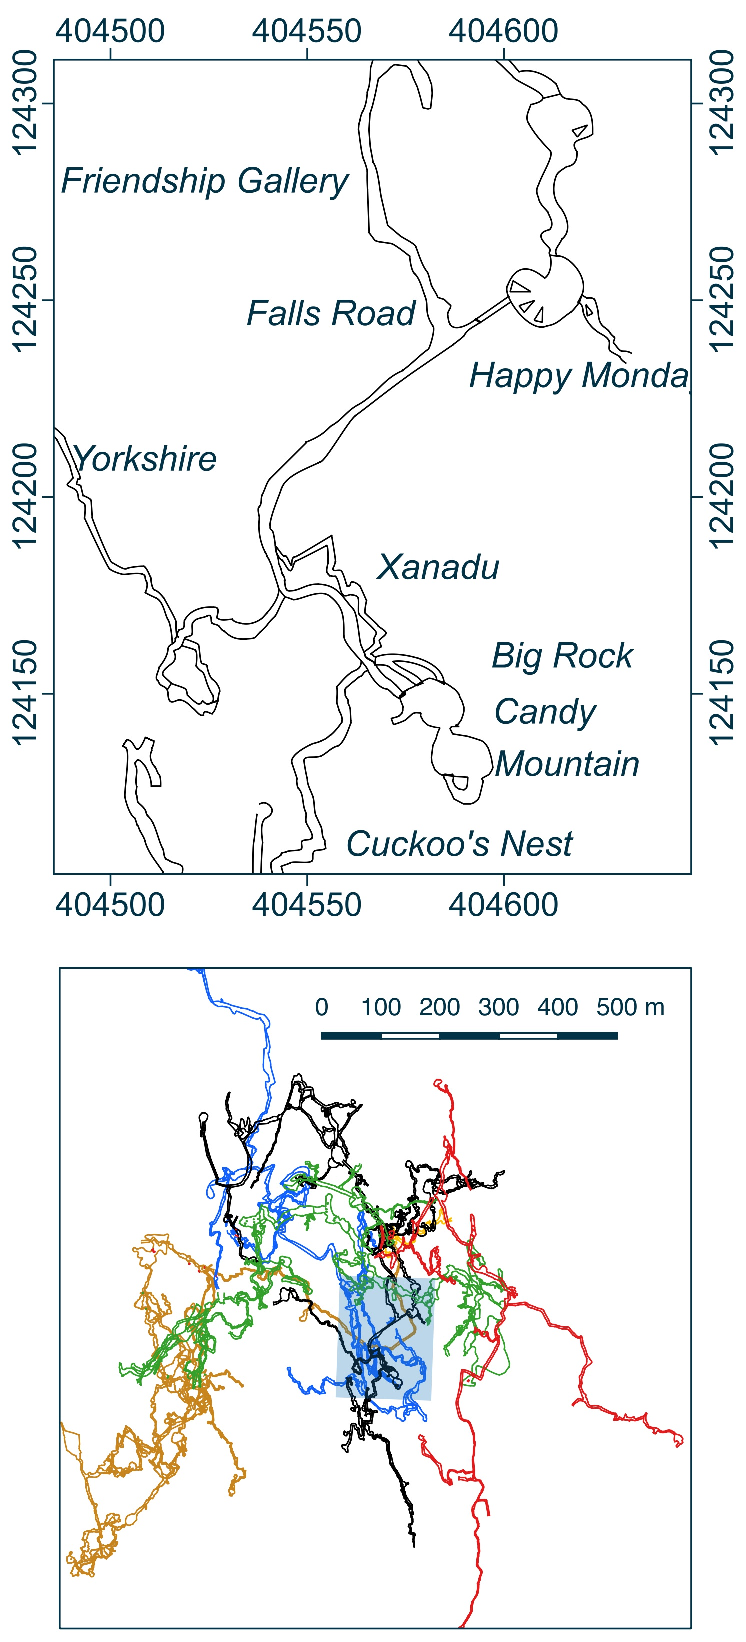
\includegraphics[width=\linewidth]{images/little_insets/bigrock_high_inset.pdf}
 \caption[Above Big Rock Candy Mountain]{Plan view of the \protect\passage{Red Cow} area and connected passages (blue) where \protect\passage[camp]{Camp Deep Core II} was set up, Slovenian National Grid ESPG 3794}
 \label{Red Cow inset}
\end{marginsurvey}


Our plan was to spend all the time near \passage{Red Cow}, emplace a tent and roll mats for a camp, get down to \passage{Watership Down} and push the dry leads near the sump, and sort out as much of the rigging between X-Ray and the sump to support a possible diving expedition next year.
After supper and a break in the weather, we set off for the cave entrance in the gathering dusk. We had two tackle sacks each.

Jarv:
\begin{citemize}
\item Daren with photo equip., survey gear, sonar + laser rangefinder, chocolate bars, music speakers. Mini Daren with drone + bike light. Additional Uneo drill and two batteries, spare 8mm bits.
\item 2 man single-skin tent, wrapped up in a roll mat
\end{citemize}

Rhys:
\begin{citemize}
\item Daren for camp with food, candles, spare batteries etc.
\item Roll mat, with a core of food packed in plastic bags and fuel for the stove.
\end{citemize}


\paragraph{Day 1}
Smooth trip down to camp, where we repacked and ate some hot food (William and Tanguy were on the day-train at a similar time, coming down to sleep then push tomorrow).
We set off with tent, roll mats and drill (with single battery), intending to stay above \passage{Republika} and sort the rigging.
The night train dragged, as it always does. The drill would not work, though we couldn't tell whether it was the (single) battery or the drill itself. Disappointing. We rebolted the freeclimb at the end of \passage{Memory Lane} with spitz.
We then progressed to \passage{Red Cow}, found a good space for the tent (slightly further along the passage, in `\passage{Nevermore}'). This is a wonderful camping spot. The passage is broad and dry (as in, oversuits seem to dry quickly there), with fine rock-flour `sand', a solid phreatic ceiling and smooth exposed rock with useful shelves. \bignote{It's particularly picturesque, with what appear to be large limpet-like fossils in the ceiling, and then a series of solution oxbows further along}.

\paragraph{The new 2-man tent at Red Cow} We located a latrine for camp, another 30m along the passage. Here a small phreatic leads down a too-small to push lead for about 5m. You could even use it as a long drop toilet, depending what you were planning to do with excrement? However, the first thing to go down it was one of my gloves (brand new, and super warm Marigold Astroflexes). I had placed them within my oversuit while cooking (to keep them warm), but forgotten about them, and then approached the latrine with sufficient momentum (and lack of care) that when I ripped open the velcro of my oversuit, one was catapulted into the breach, and I watched helplessly as it did a Jacob's ladder tumble to the 5m depths of the hole.

\begin{marginfigure}
\checkoddpage \ifoddpage \forcerectofloat \else \forceversofloat \fi
\centering
 \frame{\includegraphics[width=\linewidth]{"images/2014/jarv-2014/formations-potato".jpg}} 
 \caption{Rhys Tyers in the old sandy phreatic routes in \passage{Potato}, now with added explorer's footsteps \pic{Jarvist Frost}}
 \label{potato formations}
\end{marginfigure}

It was now approaching 4 AM and time was seriously beginning to drag. \passage{X-Ray} camp times were 8-8 this year, coming back early is extremely disruptive to the previous shift's sleep. After our coffee and lunch, we crawled into the tent (wearing full kit, minus harness and helmet) and had a little rest. Nicknamed `\passage{Camp Cuddle}' (for this year only), Rhys reckons he didn't get any sleep, but I distinctly remember him snoring.

I find it really interesting that a tent (to shield from the draft, and retain warm air) and roll mats (to insulate from the cold rock) were sufficient to make the conditions survivable (if not pleasant). Certainly we would not have been falling asleep had we been cowering in survival bags.
Anyhow, the next time I looked at my watch it was 6:30 AM and we were pretty chilled. We quickly put our gear back on, and set off at speed back towards camp. We covered the ground in 90 minutes (one bag each), moving quickly at the start as we were desperately trying to warm up!
Back at \passage{X-Ray} we were pretty exhausted. Tanguy very kindly made us tea + some supper, though neither of us were hungry ---the night train really messes up both your hunger and sleep cycles.

\paragraph{Day 2}
We packed for the depths, and figured out that it was the drill we had brought down (with dodgy wiring) rather than the batteries. William kindly carried out the dodgy drill and we packed for the bottom of the cave, with as many odd lengths of rope and sufficient hangers/bolts that we could muster. Everything was a bit minimal at \passage{X-Ray}, with fewer finds this year we hadn't seen the bulk supply of rope and equipment that occurred in previous ones. Metalwork had to be separated from bags where it was stored with carbide to keep it dry over the winter.
We went direct to \passage{Republika}, leaving the drill and food at \passage{Red Cow}, and were suitably awed by the water levels. \bignote{The chamber was very spray lashed, and a lot of water was going down the pitch -- the waterfall going directly via where the rope hung!}
So we started hand bolting to the right, avoiding the water. I put the two traverse bolts in while sucking teeth and muttering about the quality of the ceiling rock. Rhys, in his PVC, went over the edge, fixed a temporary deviation (we had no skyhook), and thereby slithered around further to the right into a cubby hole on the pitch and rigged down a dryish route, on our new 10mm gold rope. We munched a chocolate bar, and headed back to \passage{Red Cow} taking photos in \passage{Republika} and the streamway (I was very cold, Rhys was splashed after having stomped around the bottom of \passage{Republika}). This was rather difficult due to the sheer amount of spray flying about!

At \passage[camp]{Red Cow} we had a hot drink and some food. I decided the conditions really were too wet to have much of a chance of reaching the sump -- \passage{Insomnia} was likely to be wetter than \passage{Republika}, and a lot of \passage{Day Dreamers} puts you very close to the stream.

So we decided to curtail our attempt on \passage{Watership Down} for the day, and instead rig our way back to \passage{X-Ray} with the now fixed drill and battery combination. This was after another snooze at \passage{Camp Cuddle}, where \bignote{Rhys woke rather angrily after 90 minutes of sleep (when I woke I looked at my watch), believing that he'd only been in the tent five minutes!}
We collected all the 2010-2011 ropes left at \passage{Red Cow}, and returned to \passage{X-Ray} photographing and rerigging. We placed our full complement of 8 rawl bolts, forming Y-hangs where they'd been dodgy natural over-hangs, traverse lines where there were trip wires and SRT options where previously only brute force would do; and of course photographing as we went.


\begin{figure*}[t!]
\checkoddpage \ifoddpage \forcerectofloat \else \forceversofloat \fi
\centering
\frame{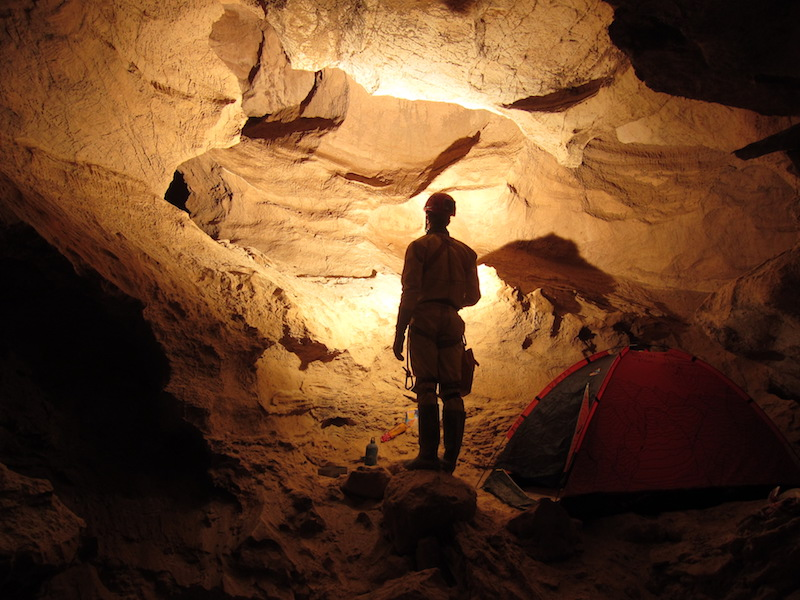
\includegraphics[width=\textwidth]{images/2014/jarv-2014/rhys_red_cow.jpg}}
\caption{Rhys Tyers at the sandy, draught-free and altogether very pleasant \protect\passage[camp]{Red Cow} camp \pic{Jarvist Frost}}
\label{rhys red cow}
\end{figure*}


\paragraph{Day 3}
During the night, Andrej and Dan arrived to visit \passage{Roaring}, but came back early at 5 and had supper then a snooze in the spare sleeping pits. When we got out of bed at 8, \passage{Zimmer} was still roaring (`like a Hydro Turbine' -- Andrej) and so we put to bed our plans to visit \passage{Watership Down}. Instead we packed laser disto, camera gear, the drone, and a proper lunch, and aimed the controls for \passage[aven]{Strap on the Nitro} (Aven) and beyond.

A speedy trip to \passage{Red Cow} admiring our new string, where we dumped the food and the stereo, pared our collection down to a single bag and continued to \passage{Strap on the Nitro}.
From \passage{Red Cow} it was up a rift to an enormous stacked boulder (I wonder if anyone dared climb past it to see if there's a continuation?) then back down to more powder-filled passage, a small pitch, an abandoned 2004 tacklesack that appeared stuffed with rope and rigging (more on this later?), and a scary freeclimb down a beautiful cliff face to reach the note demarking \passage{Strap on the Nitro}.

\begin{marginfigure}
\checkoddpage \ifoddpage \forcerectofloat \else \forceversofloat \fi
\centering
 \frame{\includegraphics[width=\linewidth]{"images/2014/jarv-2014/quadcopter-jarv".jpg}} 
 \caption{a Husban H107C HD Camera quadcopter, sealed in 3L darren drum \pic{Jarvist Frost}}
 \label{quadcopter}
\end{marginfigure}

The aven is impressive: 33m with the laser disto, smooth good quality rock at 70 degrees to the horizontal, Tetley's + Tom's escape route rigged off a nodule at about +12m, and a good draft disappearing up the aven.
We unpacked the flash and took a few photos, then got the drone out. Rhys was the WW2 `searchlight' operator with my 2xXM-L lithium ion bike light. I flew the drone.
The experience was rather exciting; control was on a knife edge. I had intended to have a few different micro-SD cards and to swap them between flights. This way if I got the beast stuck up the aven I'd still have all but the latest footage. Alas, I wasn't organised enough, so I was extremely wary of losing it.

The first flight I had a look around at up to about 20 m off the floor, checking that the controls were working. The second flight I took it straight up to near the top of the aven. Here it seemed like I was having to fight against a wind that was attempting to take me into and over to the left of the aven. Drops hitting the craft were extremely destabilising to the control system, making it pitch and precess around until recovering. After these two flights I decided we'd probably had our luck.

We then continued into \passage[|see{No More Potatoes}]{Potato} --- a lovely bit of cave with large tunnels and white powder floors, nice pitches (OK; natural belays and old 9mm again, scary). \bignote{I glanced at my watch and noticed that it was passing midnight on July 31st so I informed Rhys that his two year reign as president was over}...

\begin{quote}
`The King is dead, long live the King!'
\end{quote}

The low point you pass through (potato.23) is particular interesting, as it's got obvious features of being a river bed, with a bank of water-abraded pebbles which you crawl over.
From potato.18 you make a long and consistent assent to the end, passing over one up-pitch. The passage seems fault controlled, with sections of perfectly level bedrock.

This is the end of the 2003 pushing, and the start of \passage{Smash}. This was really quite nasty --- you start with a severe climb into an area of breakdown and boulder choke, no more white powder just angular rocks and mud. There are a few carbide arrows, but not enough to make you confident. I'm fairly certain things have moved since 2004. The area is very unstable. In the final chamber, we found the squeeze onto a pitch (blackness) which Dan had warned us about, but managed to find an earlier way through the boulders which reached a freeclimb down a steep boulder slope, to a PSS note `did you like the squeeze?'. We could see the Spitz on the wall for the squeeze then pitch, but there was no rope. This was very odd, and quite discombobulating.

\begin{marginfigure}
\checkoddpage \ifoddpage \forcerectofloat \else \forceversofloat \fi
\centering
 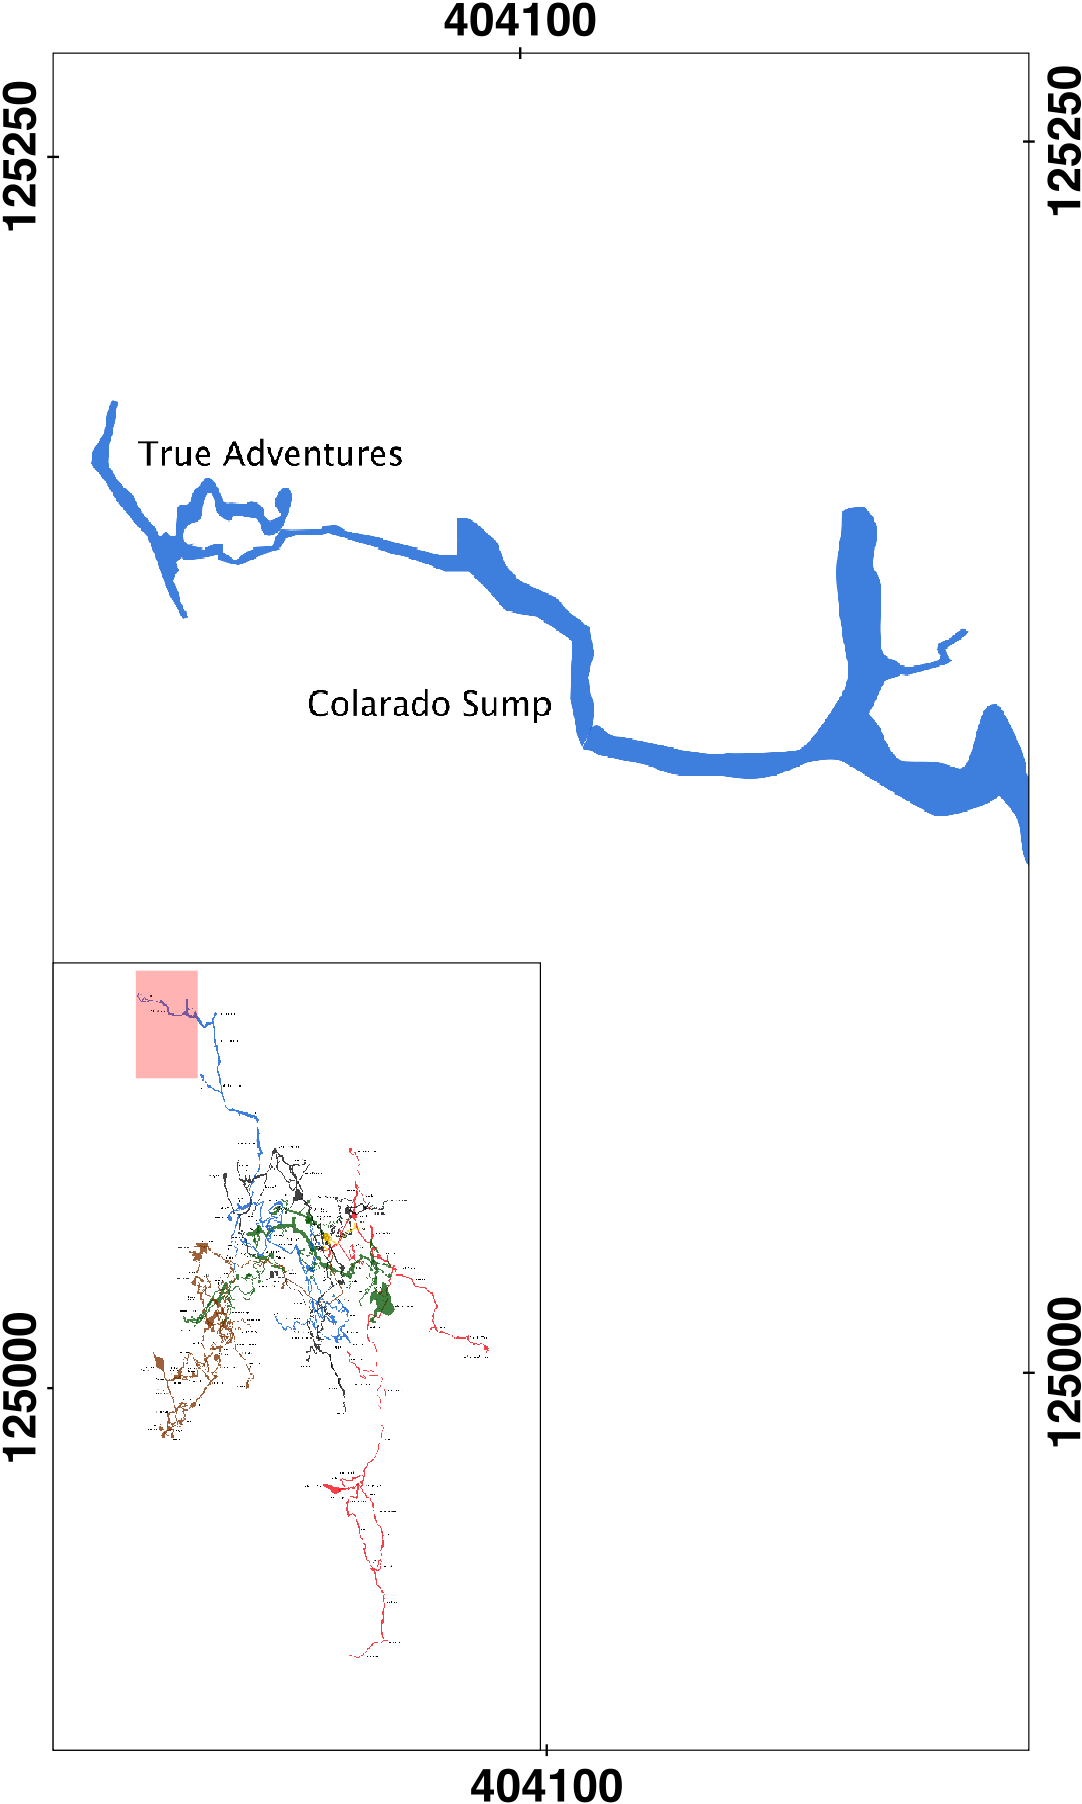
\includegraphics[width=\linewidth]{images/2014/jarv-2014/colarado_inset}
 \caption{Plan view of the \protect\passage{Colarado Sump} area visited in 2004 and 2014-15, Slovenian National Grid ESPG 3794}
 \label{colarado inset}
\end{marginfigure}

\passage{Miles Underground} was OK, being mainly wide rift passage with boulder hopping. There were a few places where you could look back + up in the rift, many possible leads. Again it wasn't super stable. It ended at a short pitch down, again derigged! The PSS talked about an undescended pitch down by a waterfall, which we could certainly hear.
Rhys found a bypass by doubling back on the right and climbing through the boulders ? tight but passable, and completely without wear.

We were now in \passage{Beyond}. After a fairly large boulder slope with the waterfall in the corner, this returned to a large-rift development, except for an obvious bit which appeared to be a fault-controlled bit of phreatic, with crack in the floor and then symmetric tulip profile either side. In a 3m wide rift we came across the \passage{Rock of Sages} -- not as big as depicted on the survey!
After more rift we reached the obvious end of \passage[|see{Infinity and Beyond}]{Beyond}. The passage just continues in rift that turns into a climb on massive blocked boulders (`\passage{To Infinity and Beyond}') though I'm not sure I would call it an aven!

The obvious way on here was a steep, again geomorphically controlled, slope of pure white limestone at about 60 deg to the horizontal and perhaps 10-15 m width. The roof was 2m away, and seemed a different, darker and more structured limestone. It was an easy descent, but I had qualms about the return.
This shallowed out into a beautiful 5 m across phreatic. After some descent, an immature stream entered on the right and started running along a 5 cm wide crack in the solid rock floor. The passage continued to a 90 degree bend to the left, where a similar sized passage issued a similarly sized stream from directly ahead. I believe this is around colarado.10 on the survey, but there were no PSS down here. I don't believe this passage has been pushed.

The combined streams continued down, and our phreatic merged with an almost identical one running in front the right, us having to step sideways between areas of boulders and confusion. (I believe this forms the `Hoover Dam', but we did not follow it).
The last run to the `sump' is absolutely dead straight (for greater than the 40 m limit of the laser disto), with about a 1 in 3 slope, and with the now 10 cm wide stream running in its own slot back and forwards across the floor. It had taken us 3.5 hours to reach \passage{Colarado} starting in \passage{X-Ray}, including playing in Strap On. Yet it felt a lot further.
The passage then flattens out, the water entering a pool mostly choked with fine rock flour which has formed a perfectly levelled silt bank which is dense enough to walk on. The PSS was on a little cairn, about 20 cm above the water level. Its pages were covered with silt deposits, but it wasn't massively disturbed, suggesting the water does occasionally backup, but never flows aggressively.

The plan shape of the passage is a hammer head, there are alcoves on the left and right with the thin crack of a fault line. The silt bank lead through a rock arch to within the `sump', so I stooped and ducked in.
\begin{figure*}[t]
\checkoddpage \ifoddpage \forcerectofloat \else \forceversofloat \fi
    \centering
    \begin{subfigure}[t]{0.345\textwidth}
    \centering
            \frame{\includegraphics[width=\linewidth]{"images/2014/jarv-2014/hourglass-passage__1_".jpg}}
        \caption{} \label{Hourglass passage}
    \end{subfigure}
        \hfill
        \begin{subfigure}[t]{0.615\textwidth}
        \centering
        \frame{\includegraphics[width=\linewidth]{"images/2014/jarv-2014/colarado_duck".jpg}}
        \caption{} \label{Colorado Duck}
    \end{subfigure}
          \vspace{0cm}
          
    \begin{subfigure}[t]{0.615\textwidth}
        \centering
        \frame{\includegraphics[width=\linewidth]{"images/2014/jarv-2014/rhys_colarado_sump".jpg}}
        \caption{} \label{Colarado Sump}
    \end{subfigure}
    \hfill
    \begin{subfigure}[t]{0.345\textwidth}
\centering
\frame{\includegraphics[width=\linewidth]{"images/2014/jarv-2014/rock-of-sages__1_".jpg}}
\label{Rock of Sages}
\end{subfigure}
    \caption{
    \textit{(a)} Passages leading to the sump, with a classic  
    \textit{(b)} A small triangular airspace beckons
    \textit{(c)}  The \protect\passage{Colarado} `duck' from higher in the passage
    \textit{(d)} The \protect\passage{Rock of Sages} \pic{Jarvist Frost}}
\end{figure*}

The first thing I noticed was the echo --- it sounded like a much larger chamber. Looking along the azure surface, there was an obvious black rock arch, seemingly about 4 m away, 40 cm across and 30 cm high above the water surface. The profile of the sump seemed to be roughly bath-tub.
I went and got camera and laser disto. By nearly touching my face to the water I could look through the arch, and see to the far side. There was a boulder at the water's edge, and slope leading up behind it. Slightly to the right of the boulder was what looked like a beach of silt or pebbles. The laser disto measured 14 m through to the other side, with 3 m from the PSS to where I was standing within the `sump'. The air was totally still, so the passage must be sumped.

From the extremely well defined 5m across phreatic, my belief is that this duck is perched, and that the phreatic has been disrupted by a slip-fault running across it. I would not be surprised if the person to first pass this duck will find a continuation of the phreatic leading down towards the water table and the terminal sump, 91 m deeper.
Certainly Rhys and I weren't seriously considering giving it a go --- we were a long way from a place of safety, where no one had been for ten years, and the navigation through \passage{Smash} and the three pitches we free climbed down were certainly weighing on my mind.

\begin{marginfigure}
\checkoddpage \ifoddpage \forcerectofloat \else \forceversofloat \fi
\centering
\frame{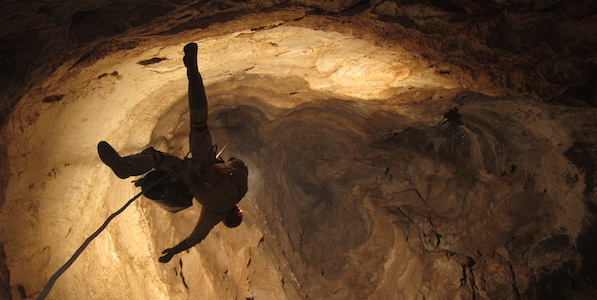
\includegraphics[height=\textwidth, angle=90]{images/2014/jarv-2014/spaceodyssey.jpg}}
\caption{The very top hang of \protect\passage{Space Odyssey}  \pic{Jarvist Frost}}
\label{SpaceOdyssey}
\end{marginfigure}

We started heading gently back, taking photos. The climb back up the steep limestone slope from \passage{Calorado Sump} was difficult. I was tall enough to push off the ceiling, where Rhys had to survive on the extremely minor footholds on the floor. Certainly it needs a rope; I think it may have been rigged with one originally, though we didn't see the Spitz.
Once back at the end of beyond, we photographed the true horror (difficult to do it justice), and free climbed up the end of the rift (\passage{Infinity and Beyond}). We stopped when we rubbed out of wear and the next boulder seemed a bit of a challenge; I think this is the exploration limit. The rift is perhaps 3-4 m wide here.

On the way back we photographed the \passage{Rock of Sages}, which Rhys stood on for the photo. He nearly got squashed by a `table top' boulder which toppled as he walked over it, dumping him against the wall and then just standing on its long edge rather than pinning him against the wall. It looked particular amusing, as the boulders here had white dustings on their tops and muddy undersides, except for the now orthogonal one.


In \passage{Smash} we were slightly stressed, both by the challenging free climb to get back into it, then a few mis turns in the boulder choke, and a TV-sized boulder that started shifting towards Rhys under my feet. We were very glad to be back in \passage{Potato} (all the 2003 cave was friendly; all the 2004 cave was scary!), where we started taking more photos.
At Red Cow we had our hot coffee, listened to some calming Ella Fitzgerald, and ate our smoked mackerel and bread / oatcake delight. We avoided \passage{Camp Cuddle}, had another hot drink and then made our slow steady way back to \passage{X-Ray}.

After a beautiful, unbroken, nights sleep we were joined by Saber and Sam. They cooked a delicious looking supper which, horrifically, was contaminated with Bitterex from the Meths. I think it must have been splashed over the packets of soup by someone refilling the Tranja. Saber made another pot of noodles, which merely tasted slightly of Petrol (probably from contamination in the Bivi).




Still feeling the weight of sleep deprivation, Rhys and I considering going out during the night, but didn't put on caving kit and in fact curled up next to Sam and Saber, and soon it was a true morning. We tidied up camp together, I had a bit of a fritz about someone having `stolen' my spare camera batteries and toothbrush, turns out that whoever they were they hid them in my resealable bag with dry socks (the fiends!), and left for the surface. Rhys and I had a full bag each (with the extra bag rolled up empty inside). On the way Rhys and I photographed from \passage[pitch]{Fistful of Tolars} to \passage{Laurel}, making an unbroken chain of photos through the cave from \passage{Colarado}.


\paragraph{Fall from Grace}
I was climbing up between one of the Urinal pitches, in an unremarkable piece of rift about a metre wide, with my arms out horizontally. Both feet slipped off their footholds at the same time, and with a terrifying grinding noise my right arm was wrenched up to the vertical. \bignote{For about half a second there was a deafening pain, and then the pain just as abruptly stopped}. I checked I could still move it, and I could! So carried on before it got too stiff. I was extremely glad I was within 40 minutes of the surface, rather than having been injured like this at the bottom. Pitch heads were rather difficult, as I couldn't lift my right arm above the horizontal, and to SRT I had to use both feet as I could no longer pull down on my hand jammer.

\begin{quote} `Hazel's not dead' \end{quote}

I exited to a total clag out, warm thick cloud enveloping the mountainside.
5PM on a Saturday; we had been underground 92 hours.

I had failed to make it down to \passage{Watership Down} (push the dry leads, and photograph the sump) ? my primary aim of the 10 days. This was the first year since 2004 in which I did not discover any new passage. But we had two full memory cards for our efforts, and some good work applied below -500 m to ease future people's work at those levels. Only one other trip had aimed to go past \passage{Red Cow} since 2004 when James KP and Dan made it to the end of \passage{Smash} before having a close shave on the squeeze-to-an-unrigged-pitch.

Sunday saw me do a down-up-down carry. My bag wasn't at all painful to carry, but I couldn't easily pick it up or put it on my shoulders! Getting into jumpers, and wriggling into sleeping bags, remains an issue.
On Sunday night I was back at \passage{Ravne} and considering how to get to \passage{Tolmin}. The light was fading, and after a brief start at walking down, I decided to take one of Tetley's bikes. I didn't have my big head lamp, just a mini single-AAA one. I considered rebuilding my caving light, but I didn't know where to find any batteries.
At the first hairpin I realised that the front disc brake was not working. This was clearly a potentially fatal issue.
I fixed it with the combi tool in the saddle bag (just needed the static pad dialing in, though it would have been a lot easier with a full size allen key!). It was now fully dark.

The descent was pretty frightening, the `Tikka' barely showed the road surface let alone warn of coming hairpins or patches of loose surface. The road is only sporadically barriered, and now that they're laying new tarmac it's not obvious whether the white is road or limestone, and whether the black is road or precipitous drops. Approaching the hydro, the brake cable came off the lever, and I barely stopped on my rear brake. I fixed this, but burnt my thumb on the rotor in the process.

Beyond the hydro, on a bend where you pass a river, there were two cold green eyes staring at me from the verge. Let's say it was a deer rather than a bear. Certainly I cycled rather quickly for the next few hundred metres.

As I approached the last long descent towards \passage{Tolmin}, heavy fat drops started to fall. I stopped next to a wood pile and repacked all my electronics in a waterproof bag. The storm broke fully and I now found myself cycling along with barely any visibility due to the torrents flying past me. Fun times.

The rain stopped by \passage{Tolmin}, and I turned up at Tetley's looking rather bedraggled, a (wiser) weaker man.

\name{Jarvist Frost}

\begin{pagefigure}
\checkoddpage \ifoddpage \forcerectofloat \else \forceversofloat \fi
\centering
 \frame{\includegraphics[width=\linewidth]{"images/2015/tanguy-lazarus-2015/jarv-sunset-2014".jpg}} 
 \caption{Catching one last sunset before leaving the expedition for this year \passage{Jarvist Frost}}
 \label{jarv sunset}
\end{pagefigure}
